\documentclass[11pt,a4paper]{article}
\usepackage[margin=19mm]{geometry}
\usepackage[T1]{fontenc}
\usepackage{lmodern}
\usepackage{microtype}
\usepackage{amsmath,amssymb}
\usepackage{xcolor}
\usepackage{tikz}
\usetikzlibrary{arrows.meta,shapes.geometric,calc}
\usepackage[hidelinks]{hyperref}

\definecolor{ink}{HTML}{243746}
\definecolor{bluewash}{HTML}{EDF4FA}
\definecolor{blueedge}{HTML}{607F99}
\definecolor{greenwash}{HTML}{EAF4ED}
\definecolor{greenedge}{HTML}{62856C}
\definecolor{rosewash}{HTML}{FAEEEE}
\definecolor{roseedge}{HTML}{A17777}
\pagestyle{plain}
\setlength{\parindent}{0pt}
\setlength{\parskip}{7pt}
\color{ink}
\newcommand{\SE}[2]{\ensuremath{#1\text{-}\mathrm{SE}_{#2}}}
\newcommand{\dual}[1]{\ensuremath{\overline{#1}}}
\tikzset{
 flow/.style={->,draw=ink},
 box/.style={rectangle,rounded corners=3pt,draw=blueedge,fill=bluewash,
     align=center,text width=5.5cm,minimum height=1cm,inner sep=6pt},
 decision/.style={diamond,aspect=2.4,draw=blueedge,fill=bluewash,
     align=center,text width=2.1cm,inner sep=3pt},
 accept/.style={box,draw=greenedge,fill=greenwash},
 reject/.style={box,draw=roseedge,fill=rosewash}
}

\begin{document}

{\LARGE\bfseries A recursive adaptive SE rule}\par
{\large Spend only the fault budget certified by the readouts}

\textbf{The earlier symmetric candidate.}
Start with \SE{Z}{d_{\rm code}}. If the readouts certify that at least $L$
internal faults have already occurred, consider the circuit label
\[
 \boxed{d_{\rm next}=\max\{1,d_{\rm code}-2L\}.}
\]
Choose the next basis separately: repeat $P$ to repair its syndrome
information, or use $\dual P$ to diagnose the other error component.
A verified branch table decides whether to correct, extract again, or discard.
The data code always keeps distance $d_{\rm code}$.

\textbf{Two different fault bounds.}
The usual correction radius is $t=\lfloor(d_{\rm code}-1)/2\rfloor$.
Our additional even-distance analysis examines histories through
$q=\lfloor d_{\rm code}/2\rfloor$ faults.
For $d_{\rm code}=4$, these are $t=1$ and $q=2$.
Thus the two-fault bound comes from this additional design contract;
it is not $(d-1)/2$ and is not a two-fault logical-correction guarantee.

\textbf{Check actions separately for X and Z.}
For each observed branch, test the correction or continuation against the
X-error condition and the Z-error condition separately. Select one action
that satisfies both. Z-SE measures the syndrome of X data errors; X-SE
measures the syndrome of Z data errors.
Use the CSS metric
\[
 \operatorname{wt}_{\rm CSS}(X(x)Z(z))=
 \max\{\operatorname{wt}(x),\operatorname{wt}(z)\}.
\]
A Y error contributes one X component and one Z component and has CSS
weight one. Keep the component fault counts separately; the physical
location count is a different quantity used by the noise model.

\textbf{A definite action need not reveal the exact fault count.}
The desired table assigns an explicit action to the available flags and
syndromes: correct, SE1, SE2, or discard. Different fault counts can lead
to the same valid action, even within a single Pauli channel.
The saved circuits provide examples [1]:

\begin{center}
\renewcommand{\arraystretch}{1.35}
\begin{tabular}{@{}lccc@{}}
\textbf{Pure faults} & \textbf{Extraction} & \textbf{Observed flags}
    & \textbf{Compatible counts}\\
\hline
Z only & \SE{Z}{4} & \texttt{00000000010} & $1$ and $2$\\
X only & \SE{X}{4} & \texttt{00000000010} & $1$ and $2$
\end{tabular}
\end{center}
In each row, the one-fault and two-fault witnesses have identical flags,
syndrome, and output Pauli modulo stabilizers. Each individual fault has a
nonzero response. No mixed X/Z history or invisible extra fault is used.
Printed strings list flag bit zero first.

This ambiguity is harmless: the same correction works for both witnesses.
It is not a circuit-distance counterexample. The numerical minimum $L$ is
used only to bound future faults when choosing a continuation; it is not
the full action or correction decoder.

\textbf{Notation throughout.}
Non-FT follow-up $=\mathrm{SE}_1$;
1-FT follow-up $=\mathrm{SE}_2$.
These are our circuit-library labels. They do not assert that a bare
syndrome-extraction circuit is a complete EC gadget.

{\footnotesize
[1] \texttt{fault\_count\_ambiguity\_checks.json}, including separate X-only
and Z-only gate-fault witnesses, each replayed with both final Bell-check
bases. The single-channel examples use one-qubit Pauli faults after gates,
at distinct gate locations. General flag-FT conditions concern compatible
corrections, not exact fault counting; see
\href{https://arxiv.org/abs/1912.09549}{Chao and Reichardt, Secs.~I--II}.
}

\clearpage
{\LARGE\bfseries The recursive presentation}\par
Let $\dual Z=X$ and $\dual X=Z$. Retain every $f_P,\sigma_P$;
use superscripts for repeated extractions. The action table and stopping
test must be certified for the complete branch. A follow-up can use the
same basis or the dual basis; see the final page.

\begin{center}
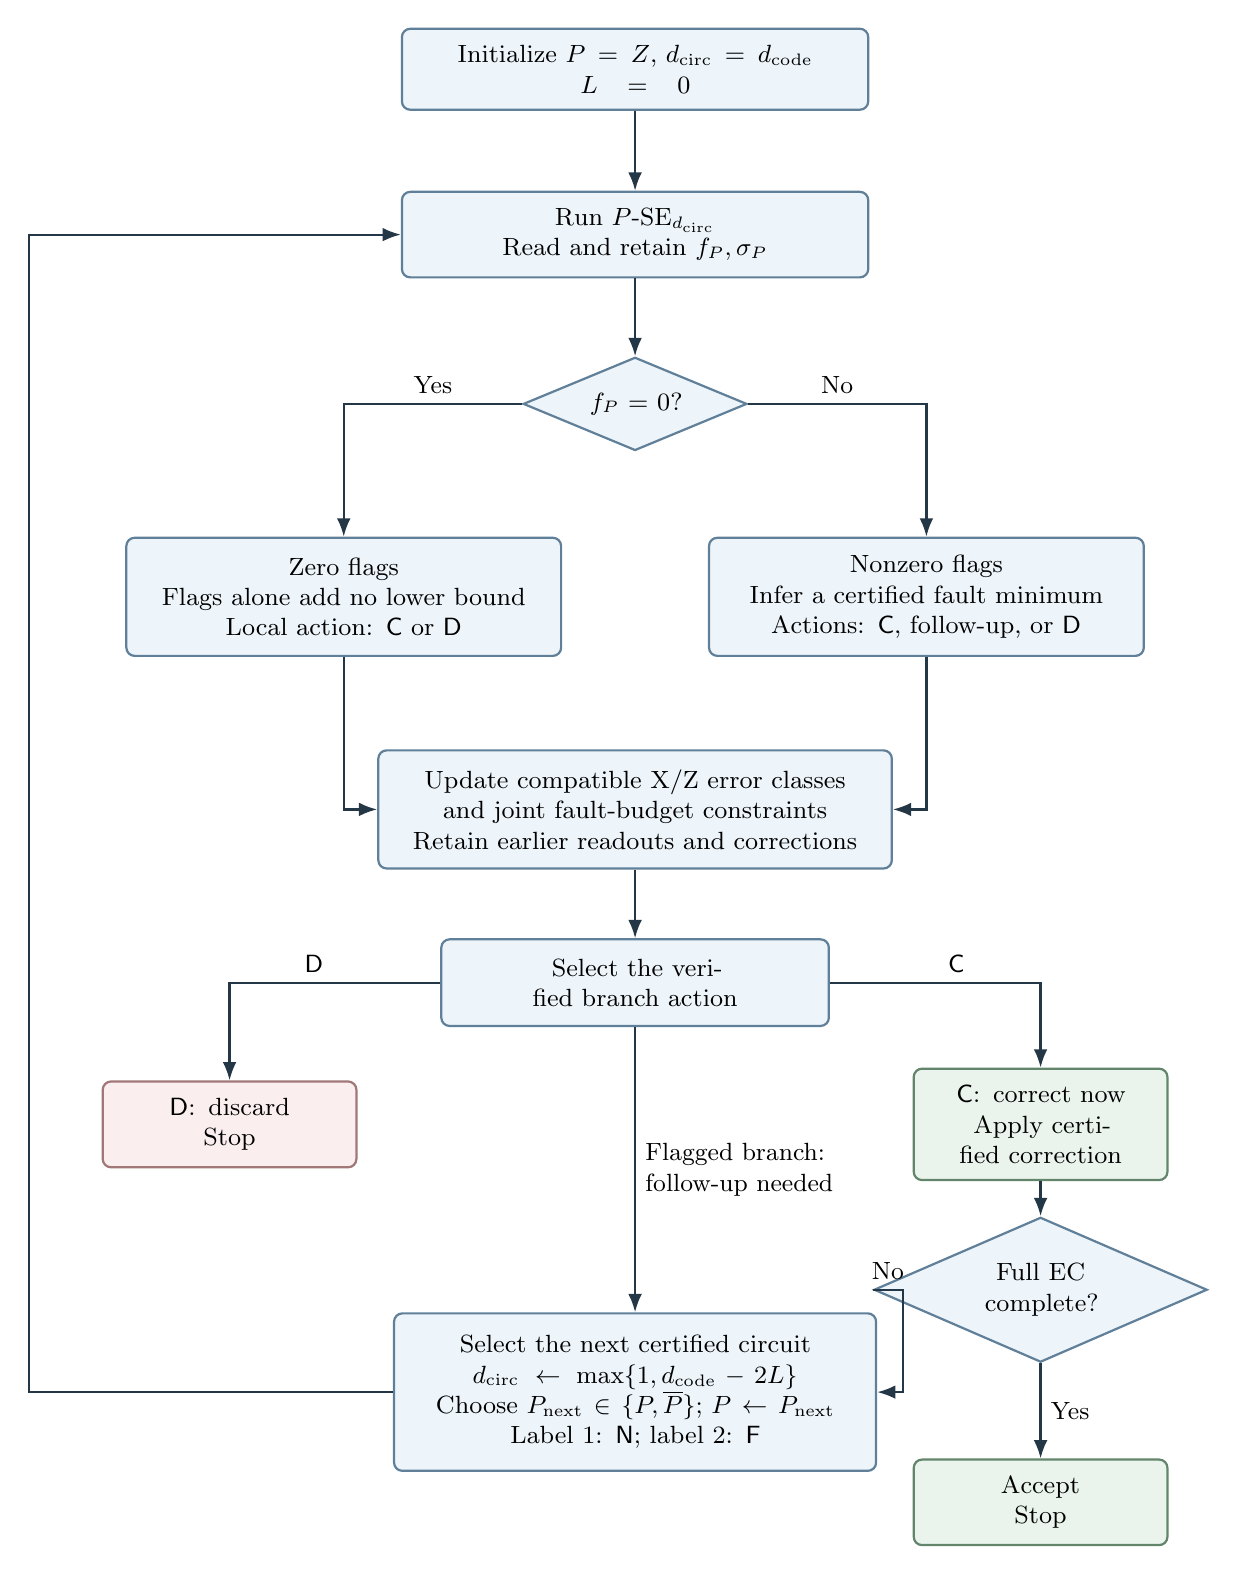
\begin{tikzpicture}[>=Latex,font=\small,line width=0.8pt]
 \node[box] (init) at (0,0)
     {Initialize $P=Z$, $d_{\rm circ}=d_{\rm code}$\\$L=0$};
 \node[box] (run) at (0,-2.1)
     {Run \SE{P}{d_{\rm circ}}\\Read and retain $f_P,\sigma_P$};
 \node[decision,text width=1.45cm] (zero) at (0,-4.25)
     {$f_P=0$?};
 \node[box,text width=5.1cm,minimum height=1.5cm] (quiet) at (-3.7,-6.7)
     {Zero flags\\Flags alone add no lower bound\\Local action: $\mathsf C$ or $\mathsf D$};
 \node[box,text width=5.1cm,minimum height=1.5cm] (flagged) at (3.7,-6.7)
     {Nonzero flags\\Infer a certified fault minimum\\Actions: $\mathsf C$, follow-up, or $\mathsf D$};
 \node[box,text width=6.1cm,minimum height=1.5cm] (update) at (0,-9.4)
     {Update compatible X/Z error classes\\and joint fault-budget constraints\\Retain earlier readouts and corrections};
 \node[box,text width=4.5cm,minimum height=1.1cm] (table) at (0,-11.6)
     {Select the verified branch action};
 \node[reject,text width=2.8cm] (discard) at (-5.15,-13.4)
     {$\mathsf D$: discard\\Stop};
 \node[accept,text width=2.8cm] (correct) at (5.15,-13.4)
     {$\mathsf C$: correct now\\Apply certified correction};
 \node[decision,text width=2cm,aspect=2.3] (done) at (5.15,-15.5)
     {Full EC\\complete?};
 \node[box,text width=5.7cm,minimum height=2cm] (next) at (0,-16.8)
     {Select the next certified circuit\\
      $d_{\rm circ}\leftarrow\max\{1,d_{\rm code}-2L\}$\\
      Choose $P_{\rm next}\in\{P,\dual P\}$; $P\leftarrow P_{\rm next}$\\
      Label $1$: $\mathsf N$; label $2$: $\mathsf F$};
 \node[accept,text width=2.8cm] (accept) at (5.15,-18.2)
     {Accept\\Stop};

 \draw[flow] (init) -- (run);
 \draw[flow] (run) -- (zero);
 \draw[flow] (zero.west) -| node[pos=0.25,above]{Yes} (quiet.north);
 \draw[flow] (zero.east) -| node[pos=0.25,above]{No} (flagged.north);
 \draw[flow] (quiet.south) |- (update.west);
 \draw[flow] (flagged.south) |- (update.east);
 \draw[flow] (update) -- (table);
 \draw[flow] (table.west) -| node[pos=0.3,above]{$\mathsf D$} (discard.north);
 \draw[flow] (table.east) -| node[pos=0.3,above]{$\mathsf C$} (correct.north);
 \draw[flow] (table.south) -- node[right,align=left]
     {Flagged branch:\\follow-up needed}
     (next.north);
 \draw[flow] (correct) -- (done);
 \draw[flow] (done) -- node[right]{Yes} (accept);
 \draw[flow] (done.west) -- (3.4,-15.5) node[midway,above]{No}
     -- (3.4,-16.8) -- (next.east);
 \draw[flow] (next.west) -- (-7.7,-16.8) -- (-7.7,-2.1) -- (run.west);
\end{tikzpicture}

{\small\textbf{Candidate recursion.} Circuit selection is repeated until a
certified correction completes EC, or a permitted discard ends the branch.}
\end{center}

After the first Z stage, $\mathsf C$ normally continues to the X stage.
At later stages it accepts only if the full EC stopping test passes.
A zero-flag syndrome that the verified stage decoder cannot correct gives
$\mathsf D$. If this would reject a guaranteed-acceptance case, the design
is infeasible and must be revised.

\clearpage
{\LARGE\bfseries What the recursion means}\par

\textbf{Use a cumulative lower bound.}
The scalar rule and example paths on this page describe the earlier
physical-location-budget candidate. They are not yet a proof for a
componentwise CSS fault budget or the asymmetric preparation below.
After extraction $j$, let $\Lambda_j$ be the set of total internal fault
counts in the observed prefix compatible with all retained readouts. Set
\[
 L_j=\min\Lambda_j.
\]
Compatibility uses the specified input and circuit-fault model and the
chosen bounded-history contract. Known corrections are included in the
prefix; faults during physical corrections count too.
An empty $\Lambda_j$ means the readouts lie outside that bounded model.
For a reachable prefix, $L_j$ cannot decrease, and at most $q-L_j$ further
internal faults remain within a total budget of $q$.

Whenever another extraction is required, propose
\[
 P_{j+1}\in\{P_j,\dual{P_j}\},\qquad
 d_{{\rm circ},j+1}=\max\{1,d_{\rm code}-2L_j\}.
\]
Choose the basis from the unresolved error or syndrome information.
All decisions use the actual readouts, not just $L_j$.

\textbf{The componentwise CSS proposal.}
Track compatible pairs $(s_X,s_Z)$ and use
\[
 s_{\rm CSS}=\max\{s_X,s_Z\}.
\]
A Y fault increments both counters by one, giving CSS fault weight one.
If the chosen contract bounds this weight by $q$, the domain is
$s_X\leq q$ and $s_Z\leq q$. It includes mixed histories at up to $2q$
distinct physical locations. An enumeration through $q$ physical faults
does not certify this entire domain. The verifier must cover these mixed
histories, directly or by a valid factorization. Physical overlap and noise
probabilities can still be retained separately. Circuit distances and the
logical-acceptance range must be checked for this explicit contract.

\textbf{Example paths at $d=4$.}
Here $\ell_i^{\min}$ is the least number of new internal faults certified
in extraction $i$. Each continuation and the final correction still require
branch verification; the required information selects the basis.
\begin{align*}
 \SE{Z}{4}&\xrightarrow{\ell_1^{\min}=0}\SE{X}{4}
     &&\text{then accept if complete},\\[4pt]
 \SE{Z}{4}&\xrightarrow{\ell_1^{\min}=1}\SE{Z}{2}
     &&\text{candidate Z-syndrome repair},\\[4pt]
 \SE{Z}{4}&\xrightarrow{\ell_1^{\min}=1}\SE{X}{2}
          \xrightarrow{\ell_2^{\min}=1}\SE{Z}{1}
     &&\text{candidate cleanup path},\\[4pt]
 \SE{Z}{4}&\xrightarrow{\ell_1^{\min}=2}\SE{X}{1}
     &&\text{no further fault budget remains}.
\end{align*}
In the cleanup chain, $L$ increases from one to two. It does not assume that
the first flag pattern identified exactly one fault. The last Z-SE1 is the
cleanup extraction: it revisits the first basis when the intervening X stage
has made that necessary. Some branches can correct and stop earlier.

\textbf{What still needs a proof.}
For each reachable branch, test all compatible inputs and fault placements
against the chosen Gottesman/CSS acceptance conditions. Include faults in
every added extraction and physical correction. Rejecting is allowed only
outside the guaranteed-acceptance regime $r+s\leq t$.

The distance update alone proves neither sufficiency nor minimality.
An earlier data error is not removed merely because a fault was counted.
A smaller circuit can be sufficient for a particular pattern; conversely,
the proposed circuit may lack necessary syndrome information. Choose a
verified continuation, or mark that branch of the proposal infeasible.
For general $d$, the required circuit labels must also exist in the library.

Finally, verify termination. Zero flags leave the flags-only distance
unchanged, and reaching SE1 is not a stopping test. Synthesize a finite
branch tree whose leaves are certified corrections or permitted discards;
otherwise even the noiseless branch could loop forever.

\clearpage
{\LARGE\bfseries Which basis should the follow-up use?}\par

\textbf{Two effects of a faulty Z extraction.}
In the Steane coupling, data $D$ controls the ancilla $A$:
\[
 \operatorname{CNOT}_{D\to A}:\qquad
 X_A\longmapsto X_A,\qquad Z_A\longmapsto Z_DZ_A.
\]
An ancilla X error at this coupling can corrupt the Z-syndrome readout
without propagating back to the data. An ancilla Z error can become a Z data
error. An X fault on the data or coupling gate can still leave an X data
error. Thus ``X faults cannot affect the data'' is too broad.

\textbf{Can the original syndrome be repaired?}
First test whether $(f_Z^x,\sigma_Z)$ already determines a common safe X
correction for every compatible history. This does not require recovering
the original error, its time, or the exact internal fault history.
Only if no such correction exists do we need additional syndrome information.

For a fixed internal fault history $F$, write
\begin{align*}
 \sigma_Z&=H_Zx_{\rm in}\oplus b_Z(F),\\
 x_{\rm out}&=x_{\rm in}\oplus a_X(F).
\end{align*}
Here $b_Z(F)$ is the shift of the recorded syndrome and $a_X(F)$ is the X
data error introduced during extraction. If the readouts uniquely determine
$b_Z(F)$, subtract it to recover the \emph{incoming syndrome}. Otherwise
the incoming syndrome remains ambiguous. Even knowing it need not identify
the original physical error or when it occurred.

In the saved circuit, the same flags \texttt{00100000000} and $\sigma_Z=31$
occur with no incoming error plus an ancilla X readout fault, or with an
incoming $X_1$ plus a flag-readout fault. The final data states differ by
$X_1$. A fault-free X-SE gives the same syndrome for both; a fault-free Z-SE
gives 0 versus 31 [2]. A noisy repeat must still be checked with the remaining
fault budget. This shows which measurement adds information, not that another
measurement is necessary: one common correction may already meet the FT bound.

\textbf{Use typed flags when their interpretation is verified.}
Write $f_Z^x$ for evidence of syndrome-corrupting X-component faults and
$f_Z^z$ for evidence of Z-component faults that can propagate to data.
For general coupling faults, retain the full response as well.
The following are candidate actions when correction or discard is not
already determined:

\begin{center}
\renewcommand{\arraystretch}{1.3}
\begin{tabular}{@{}p{4.4cm}p{5.2cm}p{5.8cm}@{}}
\textbf{Unresolved information} & \textbf{Useful extraction} & \textbf{Reason}\\
\hline
$f_Z^x$ leaves $\sigma_Z$ unreliable & Repeat \SE{Z}{\delta} & Re-measure the X-error syndrome.\\
$f_Z^z$ leaves the Z data error unknown & Use \SE{X}{\delta} & Measure the Z-error syndrome.\\
Both remain unresolved & Possibly both bases & Verify the order and shared budget.\\
Neither remains unresolved & Correct or finish the cycle & Extract only information still required.
\end{tabular}
\end{center}
Thus a full cycle may still need the dual basis after a same-basis repair.
Flags do not force an extra circuit when a safe correction is already known.

{\footnotesize
[2] \texttt{basis\_choice\_checks.json}: exact single-fault response checks
and direct replay on an encoded Bell input. In the saved basis-lowered
schedule, 10 of 11 raw flag bits can be raised by either a physical X or a
physical Z fault at different locations. Hadamards exchange these labels;
the proposed typed flags require a verified propagated-effect interpretation.
This audit does not certify the complete adaptive continuation.
}

\clearpage
{\LARGE\bfseries Alternative: asymmetric ancilla preparation}\par

\textbf{Move the retry before data coupling.}
If direct decoding from $(f_Z^x,\sigma_Z)$ is insufficient, design an ancilla
preparation with separate X and Z guarantees. Reject the preparation when
its X-side test fails, and try again before that ancilla touches the data.
An unknown Z component must either be correctable from the retained flags
or be resolved using an appropriate later X-SE measurement.

\begin{center}
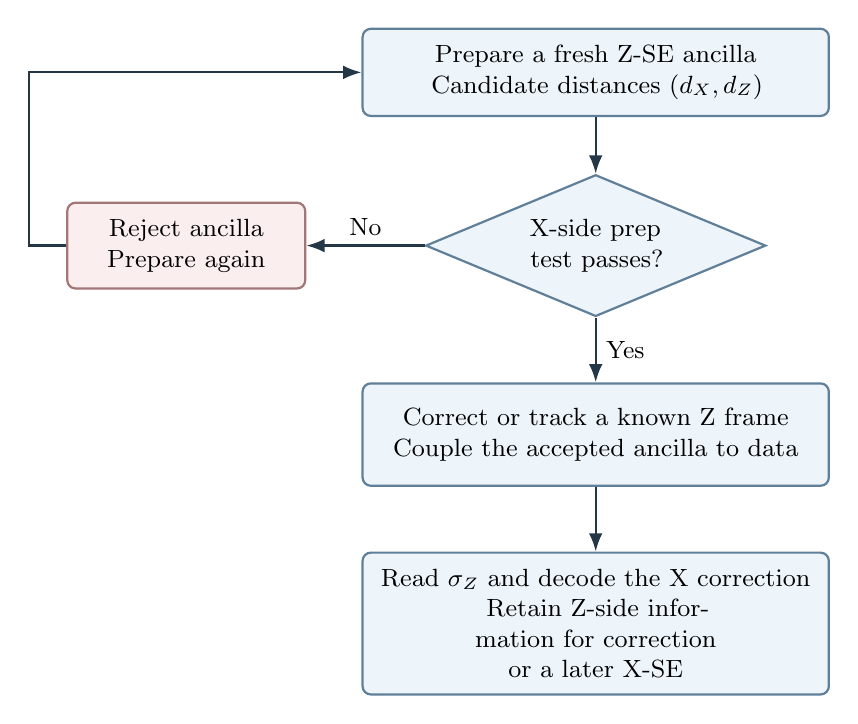
\begin{tikzpicture}[>=Latex,font=\small,line width=0.8pt]
 \node[box] (prep) at (0,0)
     {Prepare a fresh Z-SE ancilla\\Candidate distances $(d_X,d_Z)$};
 \node[decision,text width=2cm] (test) at (0,-2.2)
     {X-side prep\\test passes?};
 \node[reject,text width=2.6cm] (retry) at (-5.2,-2.2)
     {Reject ancilla\\Prepare again};
 \node[box,minimum height=1.3cm] (couple) at (0,-4.6)
     {Correct or track a known Z frame\\Couple the accepted ancilla to data};
 \node[box,minimum height=1.3cm] (read) at (0,-7.0)
     {Read $\sigma_Z$ and decode the X correction\\Retain Z-side information for correction\\or a later X-SE};
 \draw[flow] (prep) -- (test);
 \draw[flow] (test.west) -- node[above]{No} (retry.east);
 \draw[flow] (retry.west) -- (-7.2,-2.2) -- (-7.2,0) -- (prep.west);
 \draw[flow] (test) -- node[right]{Yes} (couple);
 \draw[flow] (couple) -- (read);
\end{tikzpicture}
\end{center}

\textbf{The proposed distance pair.}
For even $d=2m$, the integer interpretation is
\[
 d_X=\left\lceil\frac{d+1}{2}\right\rceil=m+1,
 \qquad d_Z=d-1=2m-1.
\]
With the usual minimum-undetectable-fault-distance meaning, $m+1$ targets
detection of harmful X faults through order $m$, while $2m-1$ targets
unique Z correction through order $m-1$. It does not promise unique
correction of every order-$m$ Z history. At $d=4$, this pair is $(3,3)$:
two-fault X detection and one-fault Z correction are distinct tasks.
For a single Z decoder, correcting one fault while detecting all incompatible
two-fault histories requires distance at least four; correcting every
two-fault history requires five. These statements concern the full relevant
readout and fault model, not a circuit filename or code-distance label.

\textbf{Prove the operational conditions.}
An accepted preparation must leave X readout corruption that the joint
decoder can safely handle, and a Z data-error class with a common valid
correction. Innocuous undetected faults need not be rejected. Include faults
in the acceptance checks, transversal coupling, measurement, and correction,
and include mixed X/Z histories under the chosen CSS budget.

This retry is different from rejecting a data block after extraction.
The saved optimized Z-SE4 interleaves preparation with data coupling:
none of its 11 flags is available before the first data interaction [2].
The proposed design therefore needs a preparation/verification barrier;
its ancilla width and waiting time must be assessed with that schedule.
Ancilla verification and retry are standard preparation tools; see
\href{https://arxiv.org/pdf/0904.2557}{Gottesman, Sec.~4.6}.

\end{document}
